\documentclass[aspectratio=169,11pt]{beamer}
\usetheme[progressbar=none,numbering=fraction,block=fill]{metropolis}
\usepackage[sfdefault,lining]{FiraSans}
\setmonofont{FiraMono-Regular.otf}[BoldFont=FiraMono-Bold.otf,Scale=MatchLowercase]
\usepackage[spanish,es-noquoting]{babel}
\usepackage{booktabs}
\usepackage{colortbl}
\usepackage{pifont}
\usepackage{appendixnumberbeamer}

\graphicspath{{../figures/}}
% colores de src/isic/plotstyle.py, para que coincidan con las figuras
\definecolor{resnet}{HTML}{1A4290}
\definecolor{effnet}{HTML}{C0392B}
\definecolor{swin}{HTML}{B8860B}
\definecolor{tinta}{HTML}{23373B}
\setbeamercolor{frametitle}{bg=tinta}
\setbeamerfont{frametitle}{size=\large}
\setbeamertemplate{frame footer}{}
\setbeamersize{text margin left=0.55cm,text margin right=0.55cm}
\makeatletter
\setlength{\metropolis@frametitle@padding}{1.5ex}
\makeatother

\newcommand{\R}{\textcolor{resnet}{\textbf{ResNet50}}}
\newcommand{\E}{\textcolor{effnet}{\textbf{EfficientNet-B0}}}
\newcommand{\Ec}{\textcolor{effnet}{\textbf{EffNet-B0}}}
\newcommand{\Sw}{\textcolor{swin}{\textbf{Swin-T}}}
\newcommand{\sd}[1]{{\scriptsize\color{gray}\,±\,#1}}
\newcommand{\hl}{\cellcolor{swin!18}}
\newcommand{\bien}{\textcolor{black!70}{\ding{51}}}
\newcommand{\mal}{\textcolor{effnet}{\ding{55}}}
\newcommand{\gc}[1]{\includegraphics[width=1.2cm]{gradcam/#1.png}}
\newcommand{\fuente}[1]{\par\vspace{2pt}{\scriptsize\color{gray}#1\par}}

\title{Comparación de ResNet50, EfficientNet-B0 y Swin-T en ISIC 2019 bajo un protocolo común}
\subtitle{Pregunta: cómo se ordenan tres arquitecturas cuando reciben exactamente el mismo presupuesto}
\author{Santiago Valdés Uriarte}
\institute{Maestría en Inteligencia Artificial y Ciencia de Datos, Universidad Panamericana\\Aprendizaje Profundo, proyecto final}
\date{15 de octubre de 2026}

\begin{document}

% 1
\begin{frame}[plain]
\titlepage
\end{frame}

% 2
\begin{frame}{Mismo protocolo para las tres arquitecturas: lo único que cambia es el modelo}
\small
\begin{columns}[T,onlytextwidth]
\column{0.47\textwidth}
\textbf{Datos: ISIC 2019}
\begin{itemize}
\item 25,331 imágenes, 8 clases
\item Desbalance de 54 a 1 (NV contra DF)
\item Partición 70/15/15 agrupada por lesión: 17,735 / 3,798 / 3,798
\item Evaluación externa: test oficial sin UNK, 6,191 imágenes
\end{itemize}
\vspace{6pt}
\begin{block}{Hardware}
RTX 5070 Ti Laptop, 12 GB de VRAM\\
Core Ultra 9, Ubuntu en WSL2
\end{block}
\column{0.49\textwidth}
\textbf{Modelos de timm, pesos de ImageNet}\par\vspace{2pt}
\begin{tabular}{lrr}
\toprule
 & Parámetros (M) & GMACs \\
\midrule
\R & 23.5 & 4.1 \\
\E & 4.0 & 0.4 \\
\Sw & 27.5 & 4.5 \\
\bottomrule
\end{tabular}
\par\vspace{6pt}
\textbf{Hiperparámetros compartidos}
\begin{itemize}
\item 224 px, AdamW con lr $10^{-4}$
\item 15 épocas, early stopping sobre F1 macro
\item Pérdida ponderada por frecuencia inversa
\item 3 semillas por modelo: 9 corridas
\end{itemize}
\end{columns}
\end{frame}

% 3
\begin{frame}{Swin-T gana en todas las métricas; en F1 macro por 5.7 pp,\\casi cuatro veces el ruido entre semillas}
\begin{columns}[T,onlytextwidth]
\column{0.45\textwidth}
\small
\setlength{\tabcolsep}{2.4pt}
\begin{tabular}{lccc}
\toprule
 & \R & \Ec & \hl\Sw \\
\midrule
\multicolumn{4}{@{}l}{\footnotesize\color{gray}Test interno (3,798)} \\
F1 macro & 52.0\sd{1.4} & 53.2\sd{0.5} & \hl\textbf{58.9}\sd{1.5} \\
Exact. bal. & 56.6\sd{1.7} & 54.1\sd{0.9} & \hl\textbf{57.7}\sd{0.9} \\
Exactitud & 65.6\sd{0.4} & 68.4\sd{0.3} & \hl\textbf{73.4}\sd{0.8} \\
AUROC & 90.7\sd{0.6} & 91.8\sd{0.1} & \hl\textbf{94.2}\sd{0.2} \\
\midrule
\multicolumn{4}{@{}l}{\footnotesize\color{gray}Test oficial (6,191)} \\
F1 macro & 51.6\sd{0.9} & 53.0\sd{1.2} & \hl\textbf{58.5}\sd{1.5} \\
\bottomrule
\end{tabular}
\fuente{En porcentaje. Media ± desviación de las semillas 0, 1 y 2.}
\column{0.53\textwidth}
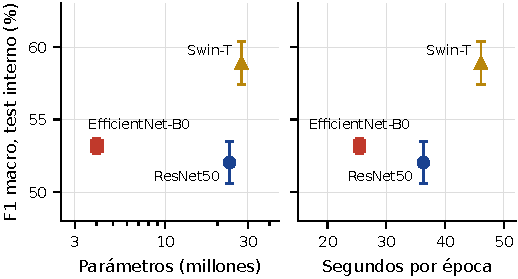
\includegraphics[width=\linewidth]{fig5_f1_vs_costo.pdf}
\fuente{F1 macro del test interno contra parámetros (escala log) y segundos por época.}
\vspace{3pt}
\small Entre las CNN el orden depende de la métrica: ResNet50 gana en exactitud balanceada.
\end{columns}
\end{frame}

% 4
\begin{frame}{Swin-T rinde más por época y EfficientNet-B0 cuesta menos;\\ResNet50 queda dominado}
\begin{columns}[T,onlytextwidth]
\column{0.505\textwidth}
\small
\setlength{\tabcolsep}{2pt}
\begin{tabular}{lccc}
\toprule
 & \R & \Ec & \Sw \\
\midrule
Parámetros (M) & 23.5 & \textbf{4.0} & 27.5 \\
GMACs & 4.1 & \textbf{0.4} & 4.5 \\
s/época & 36.3 & \textbf{25.4} & 46.1 \\
Min por corrida & 8.6 & \textbf{6.9} & 11.0 \\
VRAM (GiB) & 1.8 & \textbf{1.4} & 2.6 \\
Inferencia (img/s) & 1,770 & \textbf{3,096} & 1,189 \\
Mejor época & 10.7 & 12.3 & 13.0 \\
\bottomrule
\end{tabular}
\fuente{Media de 3 semillas. En negritas, el menor costo. Batch 32, bf16.}
\vspace{6pt}
\R\ está subajustado: F1 macro en train de 72.0, contra 90.2 y 95.5.
\column{0.475\textwidth}
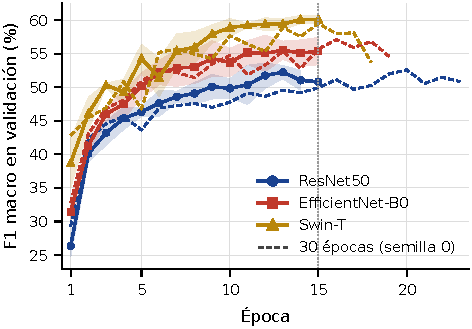
\includegraphics[width=\linewidth]{fig1_curvas_val.pdf}
\fuente{F1 macro de validación por época. Continua: media de 3 semillas. Punteada: semilla 0 con 30 épocas.}
\end{columns}
\end{frame}

% 5
\begin{frame}{El F1 macro se sostiene en el test oficial; las otras métricas caen\\de 1.7 a 4.3 pp}
\begin{columns}[T,onlytextwidth]
\column{0.49\textwidth}
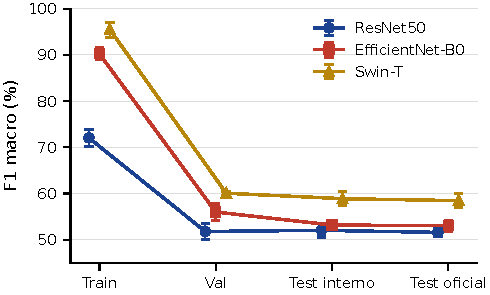
\includegraphics[width=\linewidth]{fig6_brecha_generalizacion.pdf}
\fuente{F1 macro en train (sin augmentation), validación, test interno y test oficial.}
\vspace{3pt}
\small Del interno al oficial: F1 macro, 0.4 pp o menos; exactitud balanceada, exactitud y AUROC, de 1.7 a 4.3 pp.
\column{0.49\textwidth}
\small
\setlength{\tabcolsep}{3pt}
\begin{tabular}{lccc}
\toprule
 & \multicolumn{2}{c}{F1 macro} & \\
\cmidrule(lr){2-3}
Ensemble & Interno & Oficial & GMACs \\
\midrule
\Sw\ (media) & 58.9 & 58.5 & 4.5 \\
\R\ (media) & 52.0 & 51.6 & 4.1 \\
\midrule
Arquitecturas & 59.3 & 58.2 & 9.0 \\
3 semillas \Sw & \textbf{60.5} & \textbf{60.5} & 13.5 \\
3 semillas \Ec & 56.7 & 56.9 & 1.2 \\
\bottomrule
\end{tabular}
\fuente{Promedio de softmax. Arquitecturas: semilla 0 de cada modelo.}
\vspace{3pt}
Mezclar arquitecturas no supera a 3 semillas de Swin-T; 3 EfficientNet-B0 superan a ResNet50 con menos cómputo.
\end{columns}
\end{frame}

% 6
\begin{frame}{Hipótesis descartada: sin pesos sube la exactitud y se desploma\\la exactitud balanceada}
\begin{columns}[T,onlytextwidth]
\column{0.51\textwidth}
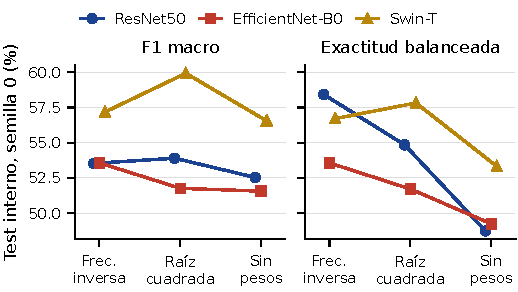
\includegraphics[width=\linewidth]{fig7_ablacion_pesos.pdf}
\fuente{Test interno, semilla 0 de cada modelo.}
\vspace{4pt}
\small Hipótesis previa: la frecuencia inversa deprime el F1 macro. Sin pesos debía subir, y baja en los tres.
\column{0.46\textwidth}
\small
\textbf{\R, semilla 0}\par\vspace{2pt}
\setlength{\tabcolsep}{3.4pt}
\begin{tabular}{lccc}
\toprule
 & Inversa & Raíz & Sin pesos \\
\midrule
F1 macro & 53.5 & 53.9 & 52.5 \\
\rowcolor{effnet!12} Exact. bal. & 58.4 & 54.8 & \textbf{48.7} \\
Exactitud & 65.9 & 70.1 & 72.7 \\
F1 macro oficial & 51.9 & 51.5 & 46.6 \\
\midrule
DF precisión & 40.4 & 27.9 & 75.0 \\
DF recall & 52.8 & 33.3 & \textbf{16.7} \\
\bottomrule
\end{tabular}
\fuente{Inversa: $1/n$ (protocolo). Raíz: $1/\sqrt{n}$. En porcentaje.}
\vspace{3pt}
Sin pesos deja de predecir las clases raras.
\end{columns}
\end{frame}

% 7
\begin{frame}{Grad-CAM permite comparar las dos CNN; en Swin-T falla el método,\\no el modelo}
\begin{columns}[T,onlytextwidth]
\column{0.47\textwidth}
\centering
\scriptsize
\setlength{\tabcolsep}{1pt}
\renewcommand{\arraystretch}{0.75}
\begin{tabular}{@{}r*{4}{c}@{}}
 & MEL & NV & BKL & DF \\
\raisebox{0.45cm}{\rotatebox{90}{Original}} & \gc{ISIC_0025800_original} & \gc{ISIC_0003462_downsampled_original} & \gc{ISIC_0026607_original} & \gc{ISIC_0069930_original} \\
\raisebox{0.3cm}{\rotatebox{90}{\textcolor{resnet}{ResNet50}}} & \gc{ISIC_0025800_resnet50} & \gc{ISIC_0003462_downsampled_resnet50} & \gc{ISIC_0026607_resnet50} & \gc{ISIC_0069930_resnet50} \\
 & SCC \mal & NV \bien & SCC \mal & DF \bien \\
\raisebox{0.4cm}{\rotatebox{90}{\textcolor{effnet}{EffNet}}} & \gc{ISIC_0025800_efficientnet_b0} & \gc{ISIC_0003462_downsampled_efficientnet_b0} & \gc{ISIC_0026607_efficientnet_b0} & \gc{ISIC_0069930_efficientnet_b0} \\
 & SCC \mal & NV \bien & NV \mal & BKL \mal \\
\raisebox{0.4cm}{\rotatebox{90}{\textcolor{swin}{Swin-T}}} & \gc{ISIC_0025800_swin_t} & \gc{ISIC_0003462_downsampled_swin_t} & \gc{ISIC_0026607_swin_t} & \gc{ISIC_0069930_swin_t} \\
 & MEL \bien & NV \bien & BCC \mal & BKL \mal \\
\end{tabular}
\column{0.50\textwidth}
\small
\textbf{CNN:} los mapas caen sobre la lesión en la mayoría de los casos y se comparan entre sí.
\par\vspace{6pt}
\textbf{Swin-T:} bloques en cruz que siguen las ventanas de $7\times7$. En el NV acierta con un mapa que cubre casi toda la imagen; en el BKL sale vacío, pues el ReLU anula un gradiente negativo.
\par\vspace{6pt}
\textbf{Lectura:} Grad-CAM se diseñó para mapas convolucionales; en Swin-T la capa objetivo es una normalización.
\fuente{Clase real como objetivo, semilla 0. Bajo cada mapa, la clase predicha. 4 de las 16 imágenes fijas.}
\end{columns}
\end{frame}

% 8
\begin{frame}{Swin-T si manda el desempeño, EfficientNet-B0 si manda el costo;\\ResNet50 no conviene con este protocolo}
\small
\begin{columns}[T,onlytextwidth]
\column{0.32\textwidth}
\textbf{Recomendación}
\begin{enumerate}
\item Sin límite de cómputo: \Sw\ (58.9; 58.5 en el oficial)
\item Hardware modesto: \E\ (0.4 GMACs, 3,096 img/s)
\item Intermedio: 3 EfficientNet-B0 (56.7 con 1.2 GMACs)
\end{enumerate}
\column{0.32\textwidth}
\textbf{Limitaciones}
\begin{enumerate}
\item Nivel bajo la literatura: 224 px, augmentation suave, 15 épocas
\item Un protocolo común no es el óptimo de cada arquitectura
\item DF y VASC con 36 y 38 imágenes de test
\end{enumerate}
\column{0.32\textwidth}
\textbf{Trabajo futuro}
\begin{enumerate}
\item Tasa de aprendizaje por arquitectura
\item Mayor resolución y preentrenamiento autosupervisado
\item Attention rollout para Swin-T
\end{enumerate}
\end{columns}
\vfill
\centering\footnotesize\color{gray} Código, configuraciones y particiones: \texttt{github.com/Valdes10U/isic2019-benchmark}
\end{frame}

\appendix

\begin{frame}[standout]
Material de respaldo
\end{frame}

\begin{frame}{Swin-T es el mejor en 7 de 8 clases; AK, SCC y DF son las más difíciles\\para los tres}
\centering
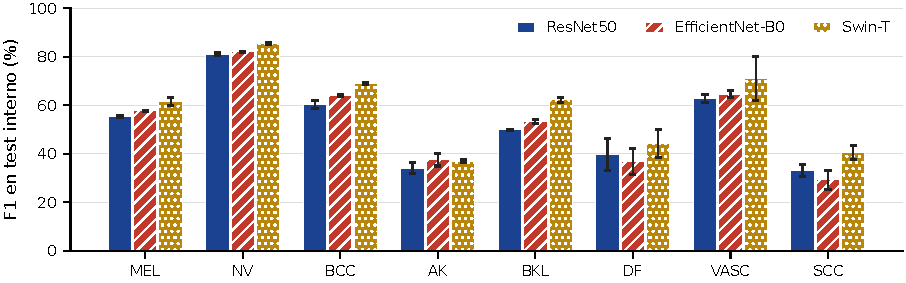
\includegraphics[width=0.7\textwidth]{fig4_f1_por_clase.pdf}
\par\vspace{2pt}
\small
\setlength{\tabcolsep}{5pt}
\begin{tabular}{lcccccccc}
\toprule
 & MEL & NV & BCC & AK & BKL & DF & VASC & SCC \\
\midrule
\R & 55.3 & 81.1 & 60.3 & 34.1 & 49.9 & 39.7 & 62.9 & 33.1 \\
\E & 57.7 & 82.1 & 63.9 & \textbf{37.6} & 53.2 & 37.0 & 64.6 & 29.3 \\
\Sw & \textbf{61.6} & \textbf{85.6} & \textbf{69.1} & 37.0 & \textbf{62.3} & \textbf{44.1} & \textbf{71.0} & \textbf{40.5} \\
\midrule
Soporte & 678 & 1,929 & 499 & 130 & 394 & 36 & 38 & 94 \\
\bottomrule
\end{tabular}
\fuente{F1 por clase en el test interno, media de 3 semillas; la desviación está en las barras de error.}
\end{frame}

\begin{frame}{Buena parte del error viene de AK y SCC confundidas con BCC,\\y de MEL confundido con NV}
\centering
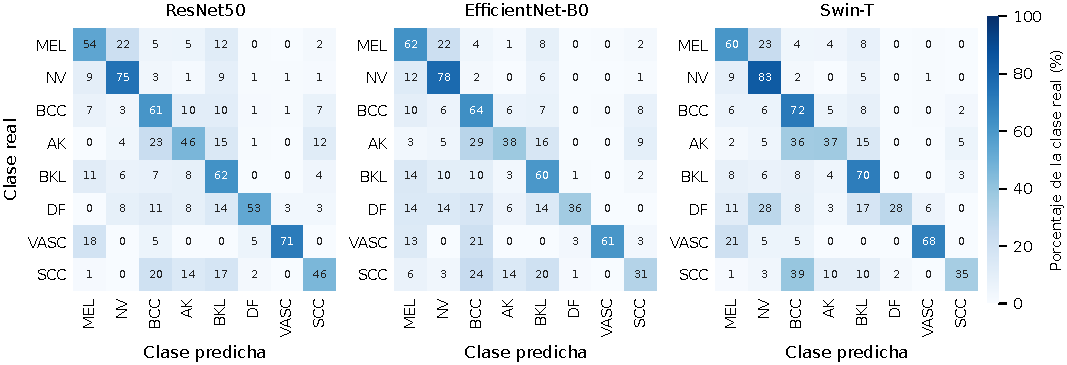
\includegraphics[width=\textwidth]{fig3_matrices_confusion.pdf}
\fuente{Test interno, semilla 0, porcentaje de cada clase real (las filas suman 100). Entre 23 y 36\% de las AK y entre 20 y 39\% de los SCC terminan en BCC; entre 22 y 23\% de los MEL, en NV.}
\end{frame}

\begin{frame}{En el test oficial la precisión de las minoritarias sube en 11 de 12 casos;\\el recall de VASC cae}
\small
\setlength{\tabcolsep}{4pt}
\begin{columns}[T,onlytextwidth]
\column{0.49\textwidth}
\begin{tabular}{lcccc}
\toprule
 & \multicolumn{2}{c}{Precisión} & \multicolumn{2}{c}{Recall} \\
\cmidrule(lr){2-3}\cmidrule(lr){4-5}
 & Interno & Oficial & Interno & Oficial \\
\midrule
\multicolumn{5}{@{}l}{\footnotesize DF (36 / 91 imágenes)} \\
\R & 36.2 & 46.2 & 45.4 & 50.2 \\
\Ec & 39.0 & 53.3 & 36.1 & 45.8 \\
\Sw & 56.5 & 78.9 & 37.0 & 49.5 \\
\midrule
\multicolumn{5}{@{}l}{\footnotesize VASC (38 / 104 imágenes)} \\
\R & 58.2 & 64.2 & 68.4 & 48.4 \\
\Ec & 64.4 & 72.1 & 64.9 & 41.0 \\
\Sw & 74.5 & 83.8 & 68.4 & 45.8 \\
\bottomrule
\end{tabular}
\column{0.49\textwidth}
\begin{tabular}{lcccc}
\toprule
 & \multicolumn{2}{c}{Precisión} & \multicolumn{2}{c}{Recall} \\
\cmidrule(lr){2-3}\cmidrule(lr){4-5}
 & Interno & Oficial & Interno & Oficial \\
\midrule
\multicolumn{5}{@{}l}{\footnotesize SCC (94 / 165 imágenes)} \\
\R & 26.7 & 28.1 & 44.7 & 38.6 \\
\Ec & 29.1 & 30.4 & 29.8 & 35.6 \\
\Sw & 49.7 & 48.8 & 34.4 & 39.4 \\
\midrule
\multicolumn{5}{@{}l}{\footnotesize AK (130 / 374 imágenes)} \\
\R & 27.3 & 29.4 & 45.6 & 38.8 \\
\Ec & 35.5 & 39.5 & 40.5 & 41.3 \\
\Sw & 36.1 & 40.9 & 37.9 & 30.4 \\
\bottomrule
\end{tabular}
\end{columns}
\fuente{En porcentaje, media de 3 semillas (desviaciones en la Tabla V del artículo). Entre paréntesis, imágenes de la clase en el test interno / oficial.}
\end{frame}

\begin{frame}{Con 30 épocas el early stopping corta antes del tope y el orden no cambia}
\centering
\setlength{\tabcolsep}{5pt}
\begin{tabular}{lcccccccc}
\toprule
 & \multicolumn{2}{c}{Época} & \multicolumn{3}{c}{F1 interno} & \multicolumn{3}{c}{F1 oficial} \\
\cmidrule(lr){2-3}\cmidrule(lr){4-6}\cmidrule(lr){7-9}
 & 15 & 30 & 15 & 30 & $\Delta$ & 15 & 30 & $\Delta$ \\
\midrule
\R & 13/15 & 20/23 & 53.5 & 54.0 & +0.5 & 51.9 & 53.0 & +1.1 \\
\E & 13/15 & 16/19 & 53.6 & 54.7 & +1.1 & 51.7 & 52.7 & +1.0 \\
\Sw & 10/13 & 15/18 & 57.2 & 60.3 & +3.1 & 57.9 & 59.1 & +1.2 \\
\bottomrule
\end{tabular}
\fuente{Semilla 0, desde ImageNet, cosine ajustado a 30 épocas (no es una continuación). Época: mejor época / épocas corridas. $\Delta$ en pp.}
\vspace{6pt}
\raggedright
\begin{itemize}
\item La ganancia de Swin-T (+3.1) se explica en parte por la semilla: la 0 era la más débil (57.2), y el 60.3 queda 1.4 pp sobre la media de 15 épocas, dentro de su desviación de 1.5.
\item ResNet50 tiene su mejor época en la 20: otra señal de subajuste.
\end{itemize}
\end{frame}

\begin{frame}{Ablación completa: la frecuencia inversa es la mejor o empata en F1 macro\\del test oficial en los tres modelos}
\centering
\scriptsize
\setlength{\tabcolsep}{2.4pt}
\begin{tabular}{llccccccccc}
\toprule
 & & \multicolumn{2}{c}{Test interno} & \multicolumn{2}{c}{Test oficial} & \multicolumn{4}{c}{Minoritarias, test interno (P / R)} \\
\cmidrule(lr){3-4}\cmidrule(lr){5-6}\cmidrule(lr){7-10}
 & Ponderación & F1 macro & Exact. bal. & F1 macro & Exact. bal. & DF & VASC & SCC & AK \\
\midrule
\R & Inversa & 53.5 & \textbf{58.4} & \textbf{51.9} & \textbf{53.2} & 40.4 / 52.8 & 58.7 / 71.1 & 29.3 / 45.7 & 26.8 / 46.2 \\
 & Raíz & \textbf{53.9} & 54.8 & 51.5 & 50.2 & 27.9 / 33.3 & 68.6 / 63.2 & 35.1 / 36.2 & 36.0 / 49.2 \\
 & Sin pesos & 52.5 & 48.7 & 46.6 & 43.7 & 75.0 / 16.7 & 90.9 / 52.6 & 26.2 / 18.1 & 38.8 / 34.6 \\
\midrule
\Ec & Inversa & \textbf{53.6} & \textbf{53.6} & \textbf{51.7} & 50.0 & 50.0 / 36.1 & 65.7 / 60.5 & 25.7 / 30.9 & 40.8 / 37.7 \\
 & Raíz & 51.8 & 51.7 & \textbf{51.7} & \textbf{50.6} & 33.3 / 22.2 & 66.7 / 63.2 & 29.3 / 38.3 & 36.8 / 30.0 \\
 & Sin pesos & 51.6 & 49.2 & 51.0 & 48.4 & 38.9 / 19.4 & 72.4 / 55.3 & 33.3 / 27.7 & 39.4 / 28.5 \\
\midrule
\Sw & Inversa & 57.2 & 56.7 & \textbf{57.9} & \textbf{55.7} & 62.5 / 27.8 & 60.5 / 68.4 & 49.3 / 35.1 & 36.1 / 36.9 \\
 & Raíz & \textbf{59.9} & \textbf{57.8} & 56.7 & 53.7 & 50.0 / 33.3 & 68.6 / 63.2 & 61.8 / 36.2 & 41.7 / 36.9 \\
 & Sin pesos & 56.5 & 53.3 & 56.6 & 53.1 & 66.7 / 22.2 & 79.3 / 60.5 & 46.4 / 34.0 & 35.0 / 33.1 \\
\bottomrule
\end{tabular}
\fuente{Semilla 0, en porcentaje. Inversa: $1/n$ (protocolo); raíz: $1/\sqrt{n}$. En negritas, la mejor variante por modelo y métrica global. El 59.9 de Swin-T con raíz iguala a su mejor semilla con frecuencia inversa.}
\end{frame}

\begin{frame}[fragile]{Las tablas y figuras se regeneran desde el repositorio en tres pasos}
\begin{columns}[T,onlytextwidth]
\column{0.40\textwidth}
\scriptsize
\begin{verbatim}
isic2019-benchmark/
  configs/   base + 1 por modelo
  src/isic/  data, models,
             train, evaluate,
             cost, ensemble,
             gradcam
  scripts/   preprocess,
             make_splits,
             run_all.sh,
             make_figures
  results/   splits y métricas
  figures/   figuras, Grad-CAM
  paper/     artículo y slides
\end{verbatim}
\column{0.58\textwidth}
\small
\textbf{Reproducir}, con los datos en \texttt{data/}:
\scriptsize
\begin{verbatim}
uv sync && uv run python scripts/preprocess.py
tmux new-session -d "bash scripts/run_all.sh"
uv run python scripts/make_figures.py
\end{verbatim}
\small
\begin{itemize}
\item 9 corridas principales: 1 h 22 min en la RTX 5070 Ti
\item Splits versionados en \texttt{results/splits/}
\item Smoke test: \texttt{isic.train -{}-smoke}
\item Pasos intermedios (evaluate, cost, ensemble, gradcam) en el README
\end{itemize}
\end{columns}
\end{frame}

\begin{frame}{Referencias clave}
\small
\begin{itemize}
\item Matsoukas et al. (2021): con pesos de ImageNet, ResNet50 y DeiT-S quedan parejos en ISIC 2019
\item Aruk, Pacal y Toprak (2026): 15 CNN contra 15 ViT en HAM10000 e ISIC 2019; Swin, la mejor exactitud
\item Ayas (2023): Swin Transformer en ISIC 2019, exactitud balanceada de 82.3
\item Gessert et al. (2020): ganador de ISIC 2019, ensembles de EfficientNets con metadata, 74.2
\item Cassidy et al. (2022): duplicados en ISIC que inflan las métricas si no se agrupa por lesión
\end{itemize}
\vfill
\scriptsize\color{gray}
Datos: ISIC 2019, licencia CC-BY-NC 4.0, sin fines comerciales.
BCN\_20000 Dataset: (c) Department of Dermatology, Hospital Clínic de Barcelona.
HAM10000 Dataset: (c) by ViDIR Group, Department of Dermatology, Medical University of Vienna; https://doi.org/10.1038/sdata.2018.161.
MSK Dataset: (c) Anonymous; https://arxiv.org/abs/1710.05006; https://arxiv.org/abs/1902.03368.
Referencias completas en \texttt{paper/articulo.pdf}.
\end{frame}

\end{document}
